\documentclass{article}%
\usepackage[T1]{fontenc}%
\usepackage[utf8]{inputenc}%
\usepackage{lmodern}%
\usepackage{textcomp}%
\usepackage{lastpage}%
\usepackage{geometry}%
\geometry{margin=0.5in}%
\usepackage{graphicx}%
%
\title{Report on WeatherAustralia dataset}%
\author{Auto2Class}%
\usepackage{amsmath}%
\usepackage{amssymb}%
\usepackage{enumitem}%
%
\begin{document}%
\normalsize%
\maketitle%
\newpage%
\tableofcontents%
\newpage%
\section{Exploratory Data Analysis}%
\label{sec:ExploratoryDataAnalysis}%
\subsection{Non{-}Null Count, Dtype of features}%
\label{subsec:Non{-}NullCount,Dtypeoffeatures}%


\begin{table}[h!]%
\caption{Dataset Columns Information}%
\vspace{0.2cm}%
\centering%
\begin{tabular}{|c||c||c||c|}%
\hline%
Index&Column&Non{-}Null Count&Dtype\\%
\hline%
0&Date&10000&object\\%
1&Location&10000&object\\%
2&MinTemp&9900&float64\\%
3&MaxTemp&9912&float64\\%
4&Rainfall&9772&float64\\%
5&Evaporation&5686&float64\\%
6&Sunshine&5152&float64\\%
7&WindGustDir&9298&object\\%
8&WindGustSpeed&9304&float64\\%
9&WindDir9am&9276&object\\%
10&WindDir3pm&9708&object\\%
11&WindSpeed9am&9875&float64\\%
12&WindSpeed3pm&9784&float64\\%
13&Humidity9am&9818&float64\\%
14&Humidity3pm&9686&float64\\%
15&Pressure9am&8940&float64\\%
16&Pressure3pm&8952&float64\\%
17&Cloud9am&6182&float64\\%
18&Cloud3pm&5960&float64\\%
19&Temp9am&9877&float64\\%
20&Temp3pm&9746&float64\\%
21&RainToday&9772&object\\%
22&RainTomorrow&9780&object\\%
\hline%
\end{tabular}%
\end{table}

%
\subsection{Descriptive Statistics}%
\label{subsec:DescriptiveStatistics}%


\begin{table}[h!]%
\caption{Dataset Descriptive Statistics}%
\vspace{0.2cm}%
\centering%
\begin{tabular}{|c||c||c||c||c||c||c||c||c||c|}%
\hline%
Index&Column Name/Statistic&count&mean&std&min&25\%&50\%&75\%&max\\%
\hline%
0&MinTemp&9900.0&12.26&6.44&{-}8.2&7.7&12.0&17.0&29.5\\%
1&MaxTemp&9912.0&23.26&7.17&{-}1.9&17.9&22.7&28.4&46.4\\%
2&Rainfall&9772.0&2.35&8.41&0.0&0.0&0.0&0.8&225.0\\%
3&Evaporation&5686.0&5.4&3.92&0.0&2.6&4.8&7.2&82.4\\%
4&Sunshine&5152.0&7.65&3.78&0.0&5.0&8.5&10.7&14.5\\%
5&WindGustSpeed&9304.0&39.95&13.45&9.0&31.0&39.0&48.0&117.0\\%
6&WindSpeed9am&9875.0&14.01&8.85&0.0&7.0&13.0&19.0&72.0\\%
7&WindSpeed3pm&9784.0&18.6&8.8&0.0&13.0&17.0&24.0&87.0\\%
8&Humidity9am&9818.0&68.89&18.88&4.0&57.0&70.0&83.0&100.0\\%
9&Humidity3pm&9686.0&51.79&20.9&2.0&37.0&52.0&66.0&100.0\\%
10&Pressure9am&8940.0&1017.68&7.08&982.2&1013.0&1017.6&1022.4&1040.4\\%
11&Pressure3pm&8952.0&1015.29&7.03&980.2&1010.5&1015.3&1020.0&1038.9\\%
12&Cloud9am&6182.0&4.44&2.88&0.0&1.0&5.0&7.0&8.0\\%
13&Cloud3pm&5960.0&4.49&2.72&0.0&2.0&5.0&7.0&8.0\\%
14&Temp9am&9877.0&17.03&6.51&{-}5.3&12.3&16.8&21.7&36.8\\%
15&Temp3pm&9746.0&21.72&6.98&{-}2.9&16.6&21.2&26.5&44.5\\%
\hline%
\end{tabular}%
\end{table}

%
\newpage%
\subsection{Distribution of features}%
\label{subsec:Distributionoffeatures}%
\subsubsection{Histograms of Numerical columns}%
\label{ssubsec:HistogramsofNumericalcolumns}%


\begin{figure}[h!]%
\centering%
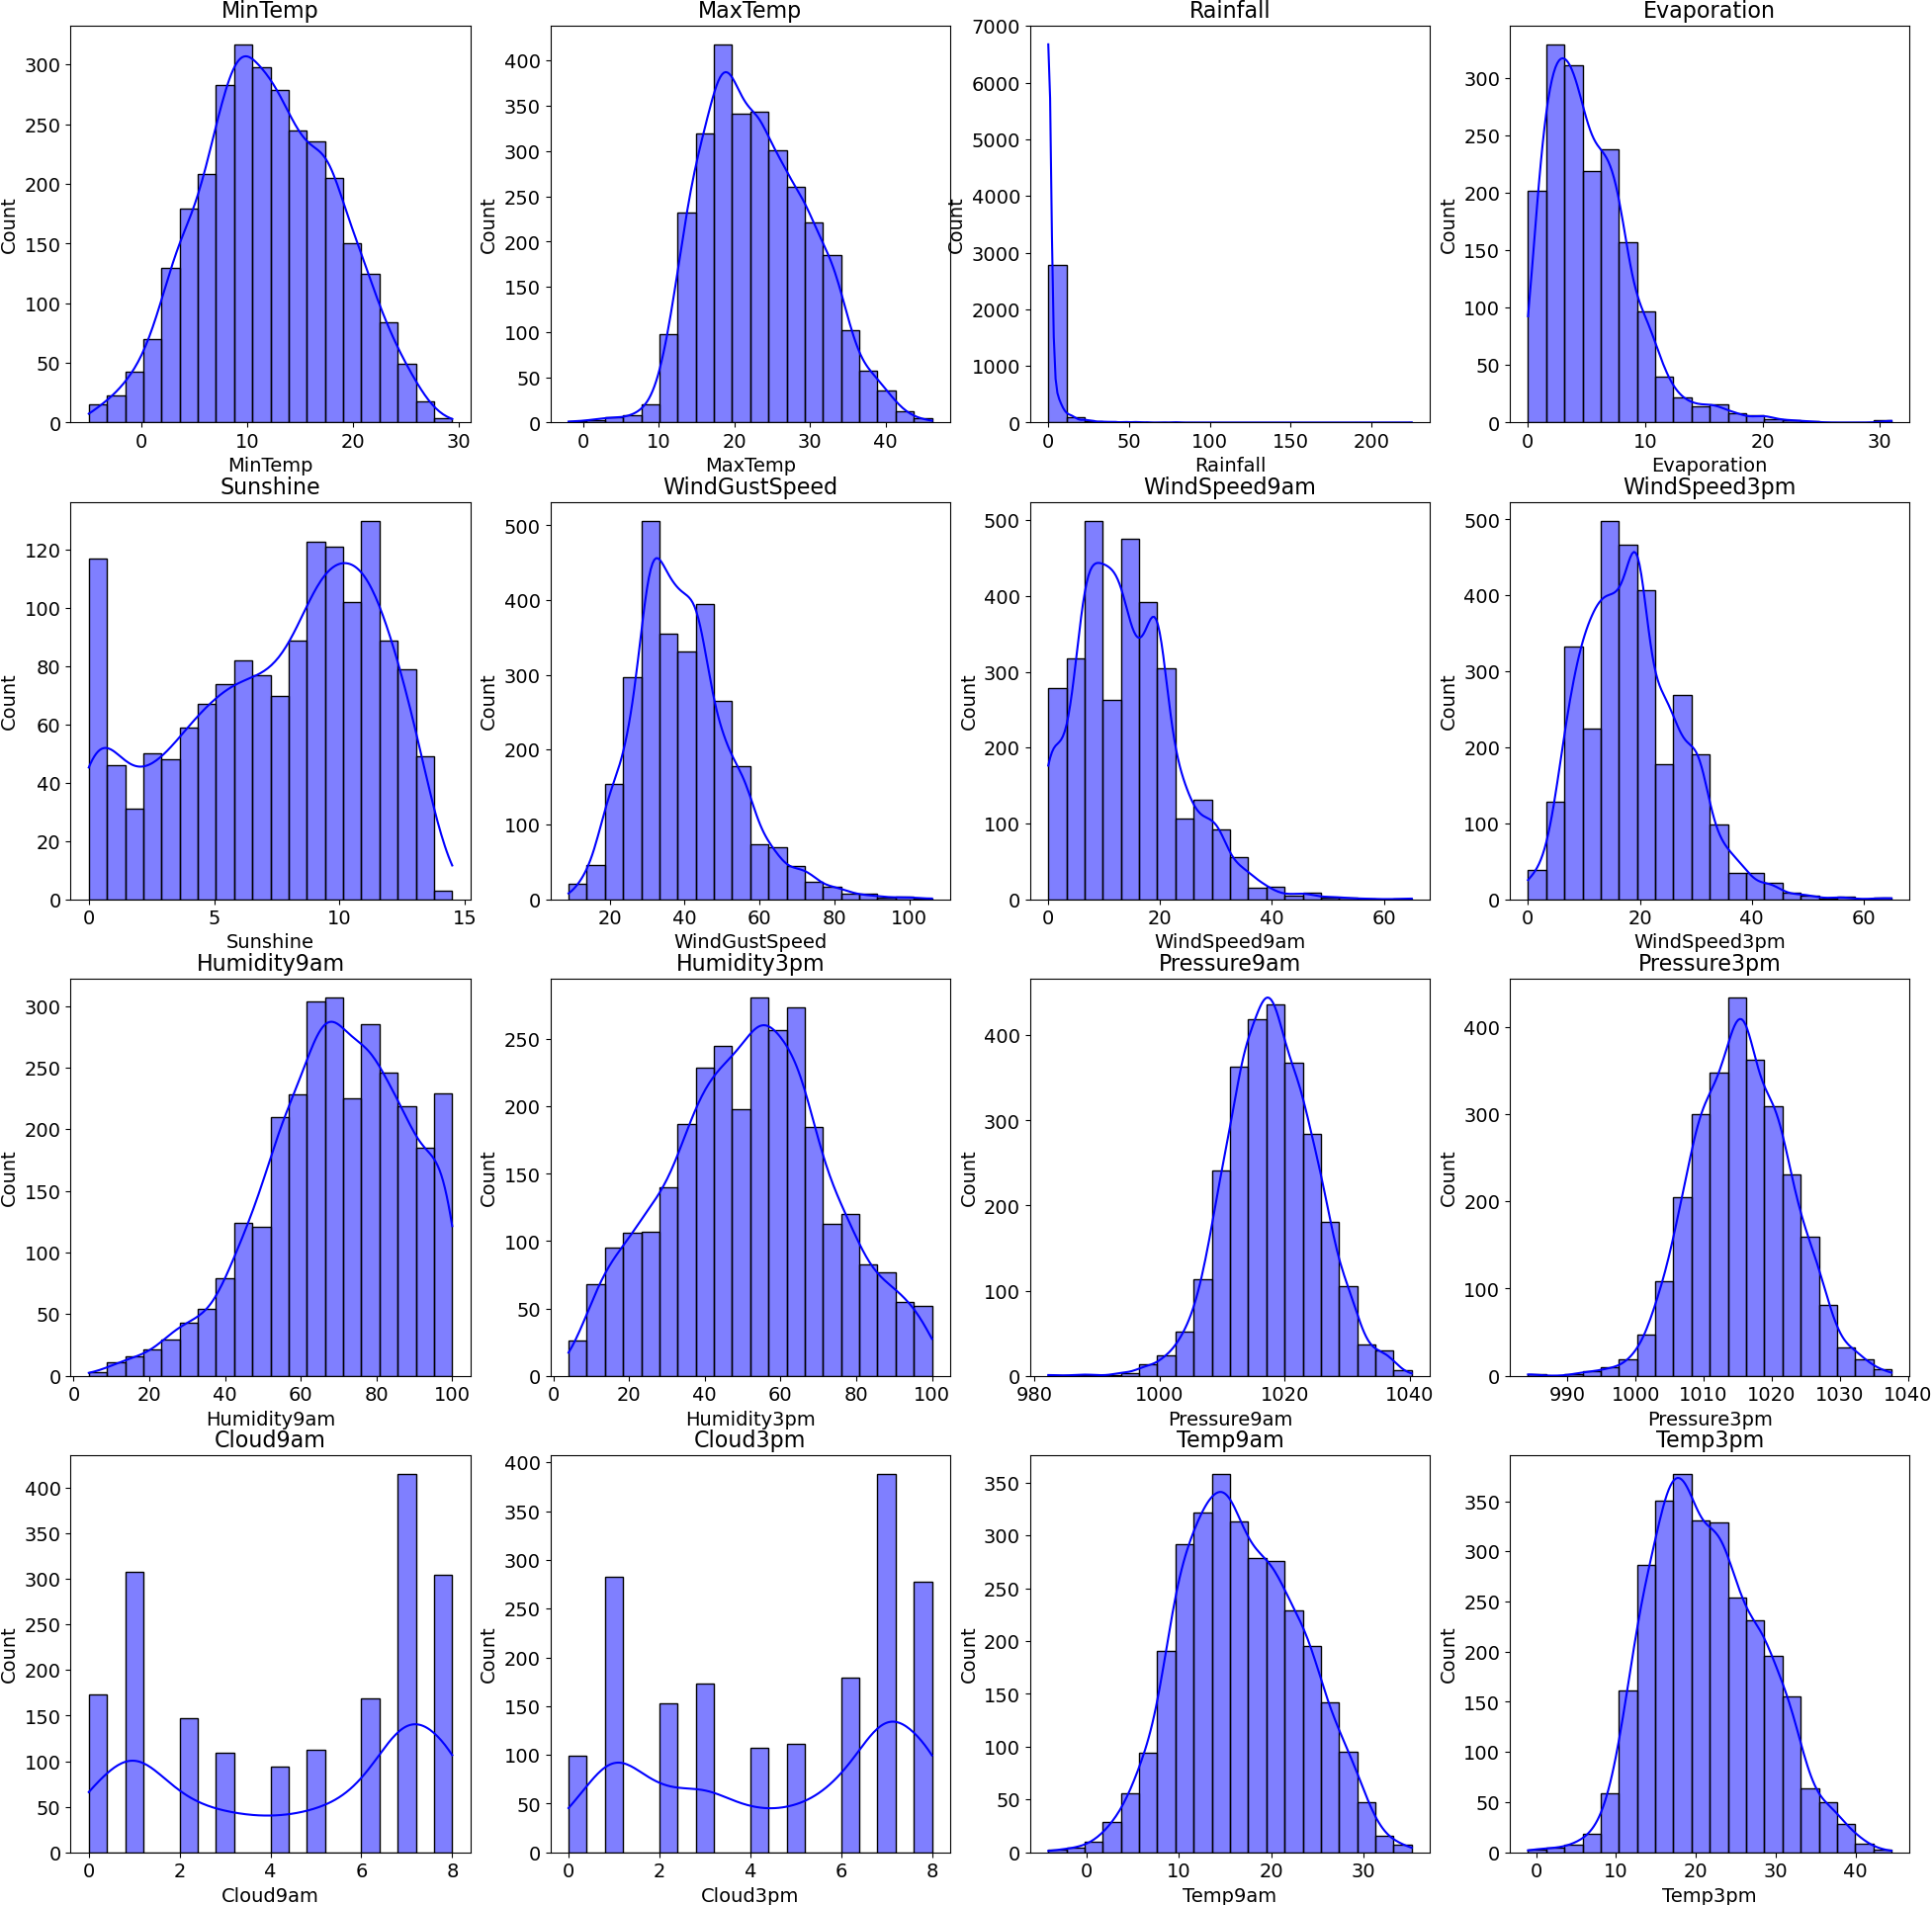
\includegraphics[width=460px]{EDA/histograms.png}%
\caption{Histograms of Numerical columns}%
\end{figure}

%
\newpage%
\subsubsection{Bar Charts of Categorical columns}%
\label{ssubsec:BarChartsofCategoricalcolumns}%


\begin{figure}[h!]%
\centering%
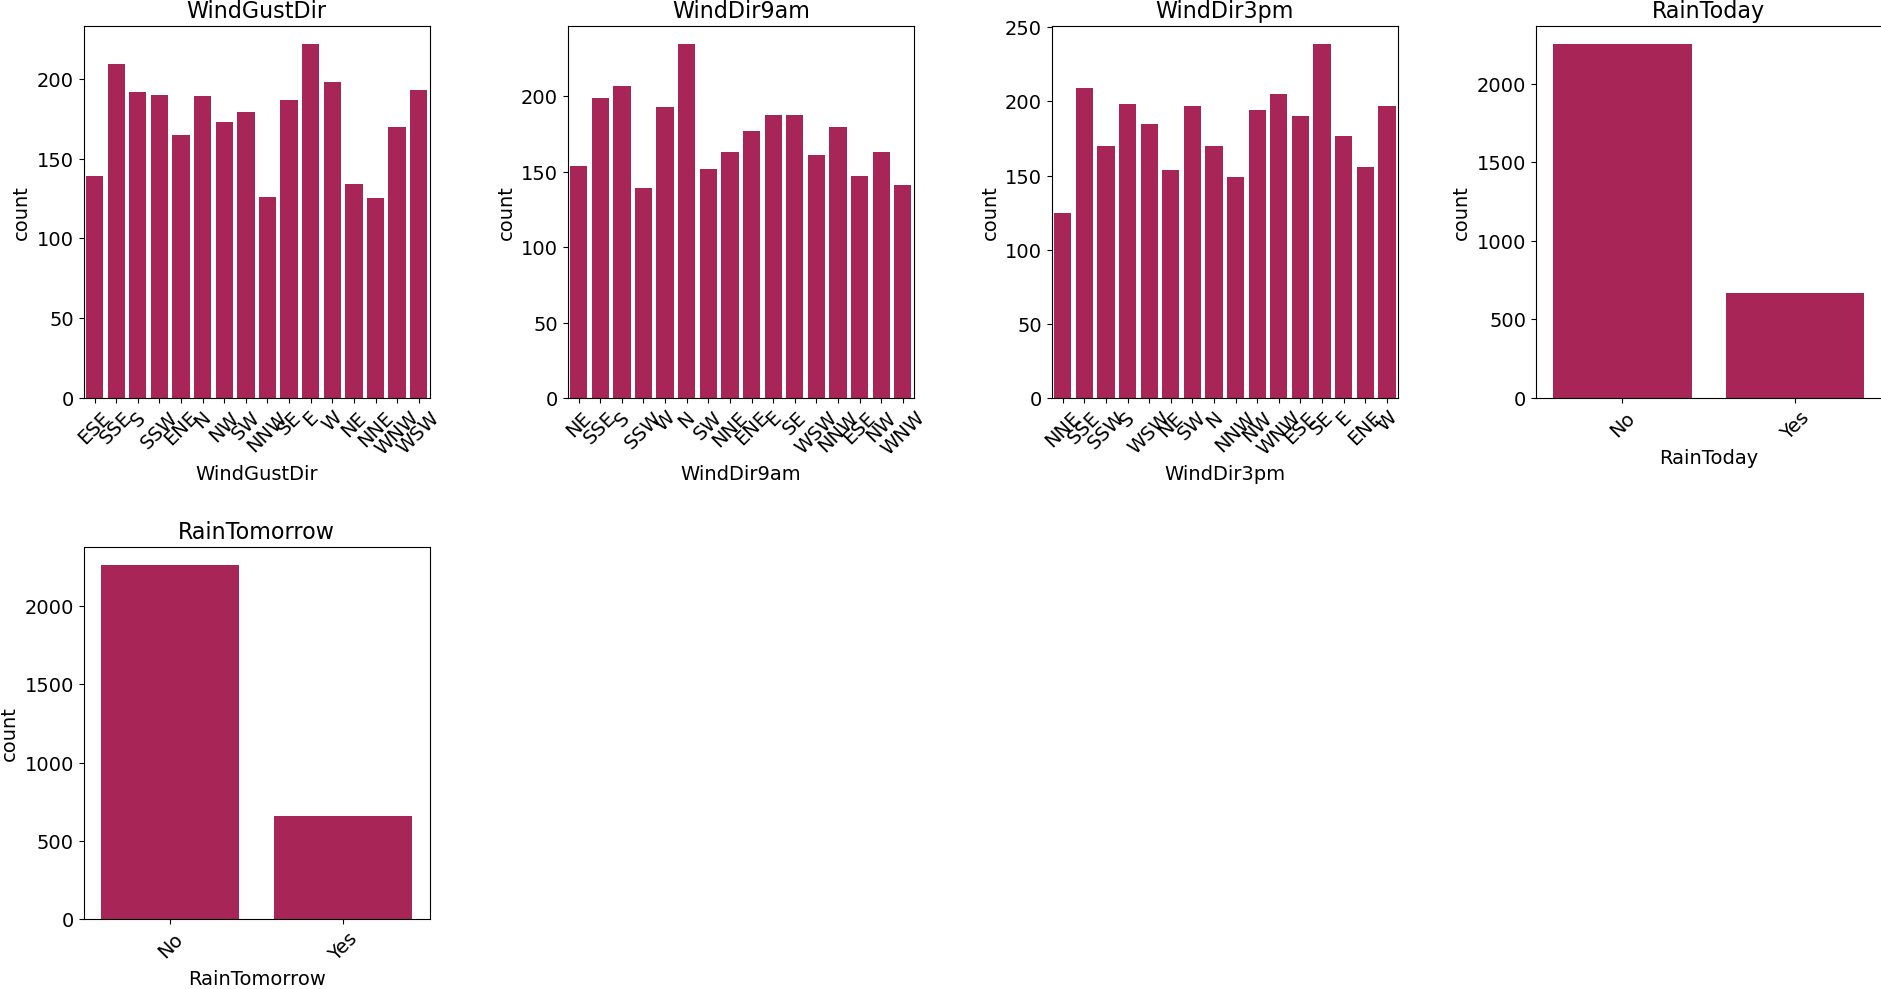
\includegraphics[width=460px]{EDA/bar_charts.png}%
\caption{Bar Charts of Categorical columns}%
\end{figure}

%
\newpage%
\section{Evaluation Metrics}%
\label{sec:EvaluationMetrics}%
\subsection{Accuracy}%
\label{subsec:Accuracy}%

                \textbf{Accuracy} is one of the simplest evaluation metrics for classification models. 
                It is defined as the ratio of correctly predicted observations to the total number of observations:

                \[
                \text{Accuracy} = \frac{\text{Number of Correct Predictions}}{\text{Total Number of Predictions}}
                \]

                While accuracy is intuitive and easy to understand, it may not be suitable for imbalanced datasets. 
                For example, in a dataset where 95\% of the samples belong to one class, predicting the majority class for every instance 
                would result in high accuracy but poor performance on the minority class.
                

%
\subsection{F1 Score}%
\label{subsec:F1Score}%

                The \textbf{F1 Score} is the harmonic mean of Precision and Recall, providing a balance between the two. 
                It is particularly useful when dealing with imbalanced datasets. Precision and Recall are defined as follows:

                \[
                \text{Precision} = \frac{\text{True Positives}}{\text{True Positives} + \text{False Positives}}
                \]
                \[
                \text{Recall} = \frac{\text{True Positives}}{\text{True Positives} + \text{False Negatives}}
                \]

                The F1 Score combines these metrics:

                \[
                \text{F1 Score} = 2 \cdot \frac{\text{Precision} \cdot \text{Recall}}{\text{Precision} + \text{Recall}}
                \]

                A high F1 Score indicates a good balance between Precision and Recall, making it a valuable metric in scenarios where false positives 
                and false negatives have significant costs.
                

%
\subsection{ROC AUC}%
\label{subsec:ROCAUC}%

                The Receiver Operating Characteristic (ROC) curve plots the True Positive Rate (Recall) against the False Positive Rate at various threshold settings. 
                The \textbf{Area Under the Curve (AUC) of the ROC curve} measures the overall ability of the model to distinguish between classes. 

                \[
                \text{AUC} = \int_{\text{FPR}=0}^{1} \text{TPR}(\text{FPR}) \, d(\text{FPR})
                \]

                Key points about ROC AUC:
                \begin{itemize}
                    \item An AUC of 0.5 indicates random guessing.
                    \item An AUC of 1.0 indicates perfect classification.
                    \item It is a threshold-independent metric, providing an aggregate measure of performance across all classification thresholds.
                \end{itemize}

                ROC AUC is particularly useful for binary classification tasks and provides insights into the trade-off between sensitivity and specificity.
                

%
\newpage%
\section{Model Optimization Results}%
\label{sec:ModelOptimizationResults}%
\subsection{Optimization Results Tables}%
\label{subsec:OptimizationResultsTables}%


\begin{table}[h!]%
\caption{Random Forest Hyperparameters and achivied metrics}%
\vspace{0.2cm}%
\centering%
\begin{tabular}{|c||c||c||c||c||c||c||c||c||c|}%
\hline%
Index&Metric/Hyperp.\textbackslash{} Iteration&0&1&2&3&4&5&6&7\\%
\hline%
0&f1&0.9386&0.7892&0.9316&0.7389&0.7581&0.9506&0.735&0.8504\\%
1&accuracy&0.9387&0.7892&0.9317&0.739&0.7581&0.9506&0.735&0.8504\\%
2&roc\_auc&0.988&0.8731&0.9867&0.8102&0.8435&0.9897&0.8108&0.9282\\%
3&n\_estimators&100&50&50&50&200&100&200&200\\%
4&criterion&gini&gini&log\_loss&log\_loss&gini&entropy&gini&log\_loss\\%
5&max\_depth&None&20&30&10&10&None&30&10\\%
6&min\_samples\_split&2&2&2&10&10&2&10&10\\%
7&min\_samples\_leaf&1&1&1&4&2&2&1&1\\%
8&min\_weight\_fraction\_leaf&0.0&0.01&0.0&0.1&0.05&0.0&0.1&0.0\\%
9&max\_features&sqrt&log2&None&None&sqrt&sqrt&None&log2\\%
10&bootstrap&1&1&1&0&1&0&0&1\\%
\hline%
\end{tabular}%
\end{table}

%


\begin{table}[h!]%
\caption{Decision Tree Hyperparameters and achivied metrics}%
\vspace{0.2cm}%
\centering%
\begin{tabular}{|c||c||c||c||c||c||c||c||c||c|}%
\hline%
Index&Metric/Hyperp. \textbackslash{} Iteration&0&1&2&3&4&5&6&7\\%
\hline%
0&f1&0.8973&0.7176&0.8504&0.7304&0.5374&0.8137&0.8654&0.4482\\%
1&accuracy&0.8979&0.7226&0.8508&0.7306&0.5835&0.8138&0.8658&0.4978\\%
2&roc\_auc&0.8979&0.7166&0.8991&0.7826&0.6173&0.8845&0.8951&0.4994\\%
3&criterion&gini&log\_loss&log\_loss&gini&gini&entropy&entropy&entropy\\%
4&splitter&best&best&best&best&random&best&random&best\\%
5&max\_depth&None&None&40&10&40&10&40&40\\%
6&min\_samples\_split&2&10&2&10&5&5&5&5\\%
7&min\_samples\_leaf&1&2&4&4&1&1&1&4\\%
8&max\_features&None&None&sqrt&None&None&None&log2&log2\\%
9&class\_weight&None&None&None&None&balanced&balanced&balanced&balanced\\%
10&min\_impurity\_decrease&0.0&0.1&0.0&0.01&0.05&0.0&0.0&0.1\\%
\hline%
\end{tabular}%
\end{table}

%


\begin{table}[h!]%
\caption{XGBoost Hyperparameters and achivied metrics}%
\vspace{0.2cm}%
\centering%
\begin{tabular}{|c||c||c||c|}%
\hline%
Index&Metric/Hyperp. \textbackslash{} Iteration&0&1\\%
\hline%
0&f1&0.9187&0.8807\\%
1&accuracy&0.9188&0.8807\\%
2&roc\_auc&0.9674&0.9489\\%
3&eval\_metric&logloss&logloss\\%
4&n\_estimators&100&50\\%
5&max\_depth&6&10\\%
6&learning\_rate&0.3&0.05\\%
7&subsample&1.0&0.7\\%
8&colsample\_bytree&1.0&0.7\\%
9&min\_child\_weight&1&1\\%
10&gamma&0&0\\%
11&reg\_alpha&0&1\\%
12&reg\_lambda&1&1\\%
\hline%
\end{tabular}%
\end{table}

%
\newpage%
\subsection{Boxplots of accuracy, f1, roc\_auc}%
\label{subsec:Boxplotsofaccuracy,f1,rocauc}%


\begin{figure}[h!]%
\centering%
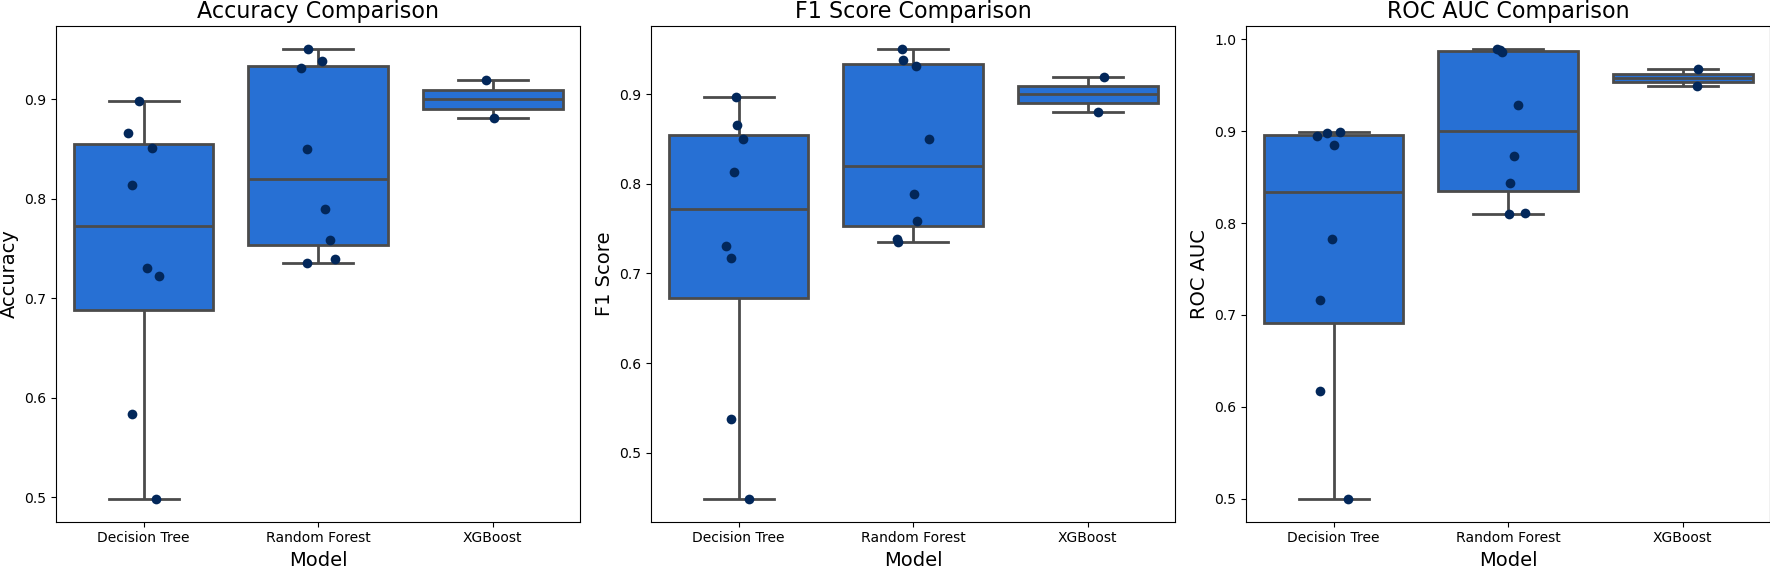
\includegraphics[width=460px]{ModelOptimization/box_plots_metrics.png}%
\caption{Boxplots of accuracy, f1, roc\_auc}%
\end{figure}

%
\subsection{Barplots of maximum values of metrics achievied by model}%
\label{subsec:Barplotsofmaximumvaluesofmetricsachieviedbymodel}%


\begin{figure}[h!]%
\centering%
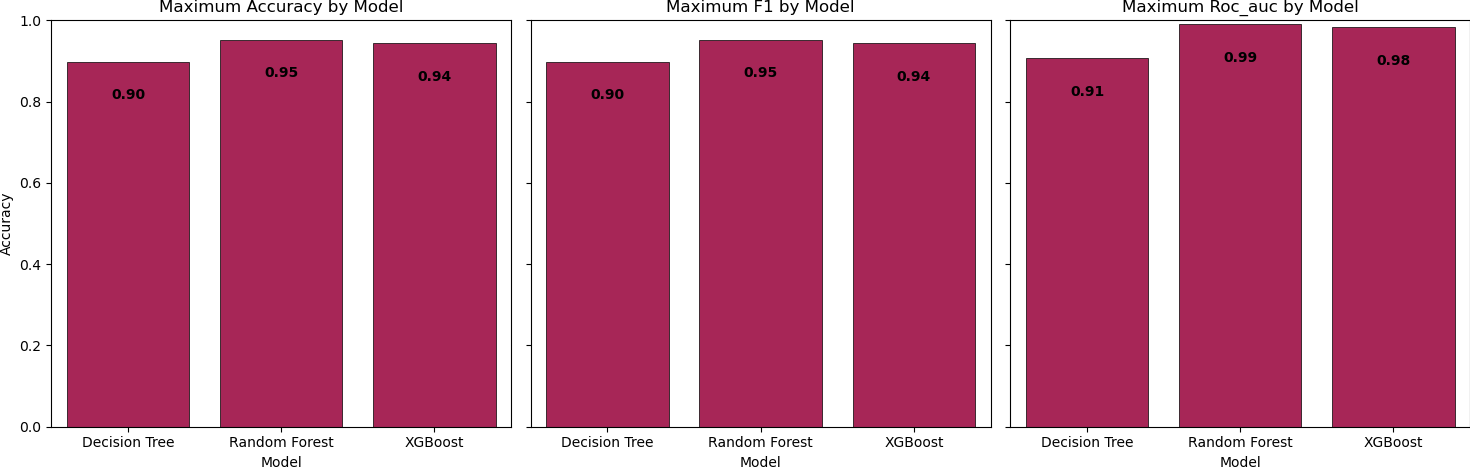
\includegraphics[width=460px]{ModelOptimization/barplots_max_metric.png}%
\caption{Barplots of maximum values of metrics achievied by model}%
\end{figure}

%
\newpage%
\section{Interpretabilty of the best models}%
\label{sec:Interpretabiltyofthebestmodels}%
Auto2class package defined the best model as the one that achievied the highest value of a metric, chosen by the user, or ROC AUC by default.%
In this case, the optimization process was aimed at maximizing%
\textbf{ ROC AUC.}%
\\%
Do not forget, that after preprocessing, columns names have changed, because of transformations of categorical features.%
\subsection{The best XGBoost model Explanation}%
\label{subsec:ThebestXGBoostmodelExplanation}%


\begin{figure}[h!]%
\centering%
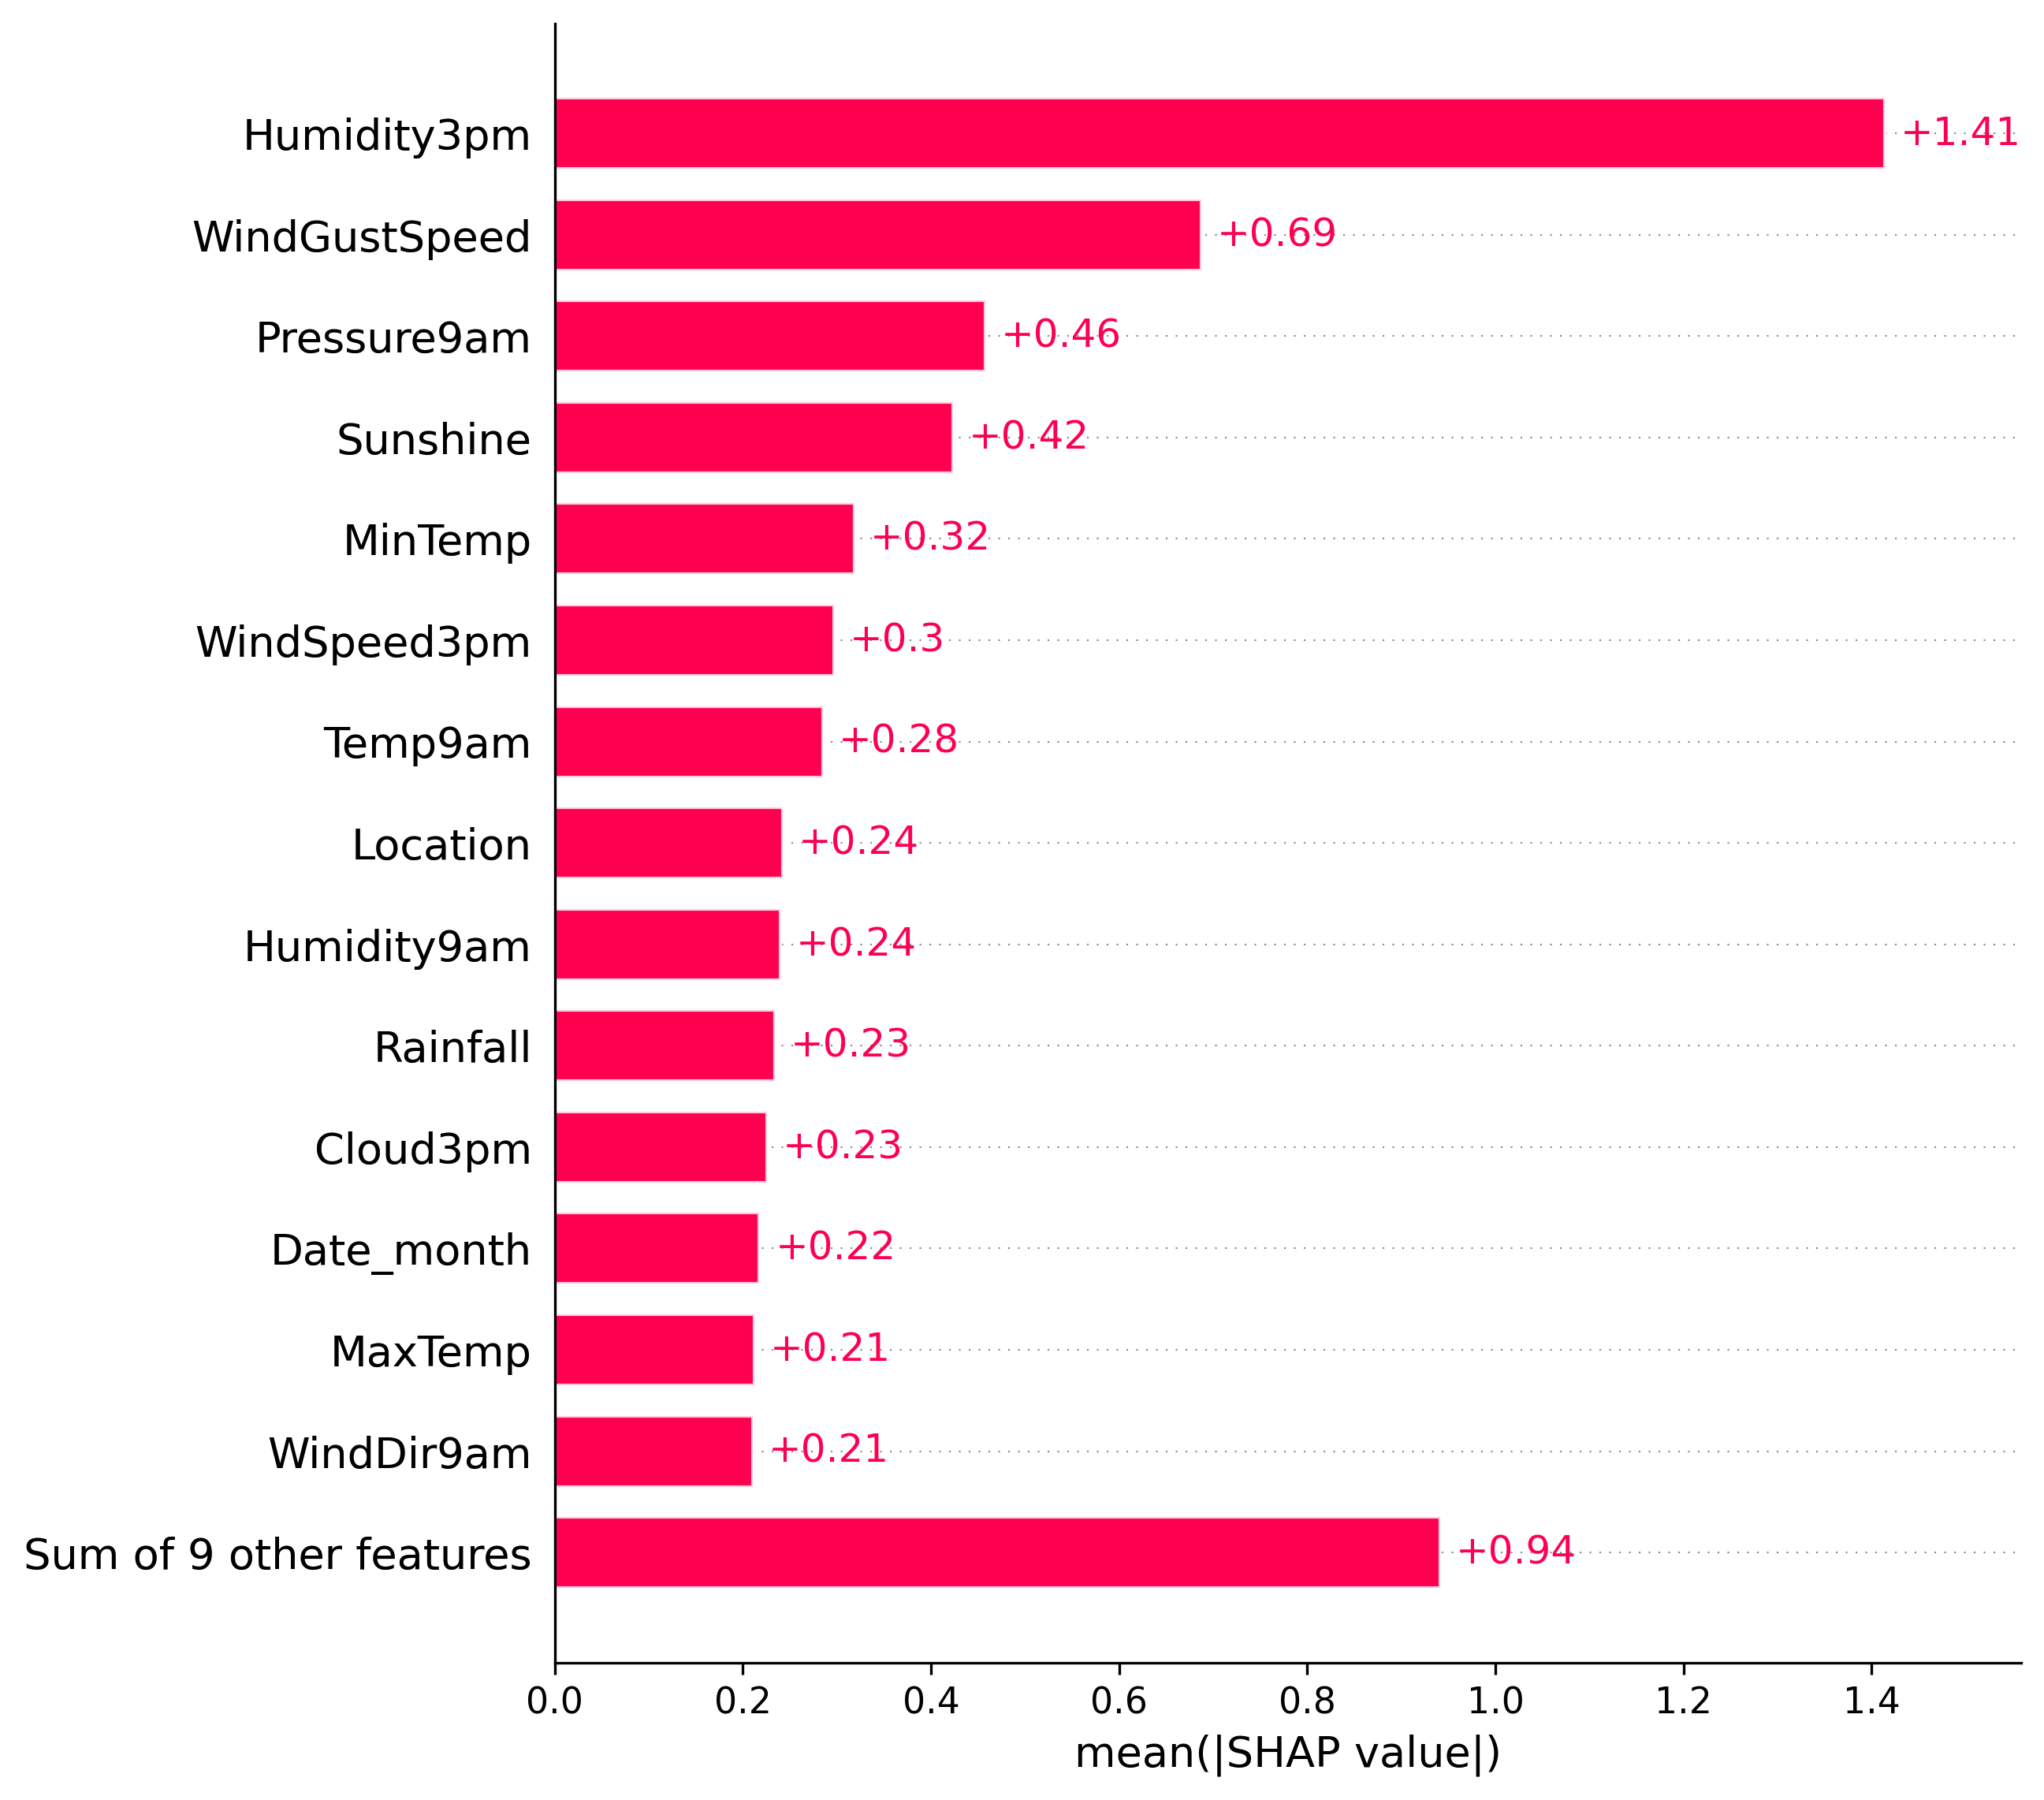
\includegraphics[width=350px]{XAI/XGBoost/global_feature_importance_shap.png}%
\caption{SHAP values for the best XGBoost model}%
\end{figure}

%


\begin{figure}[h!]%
\centering%
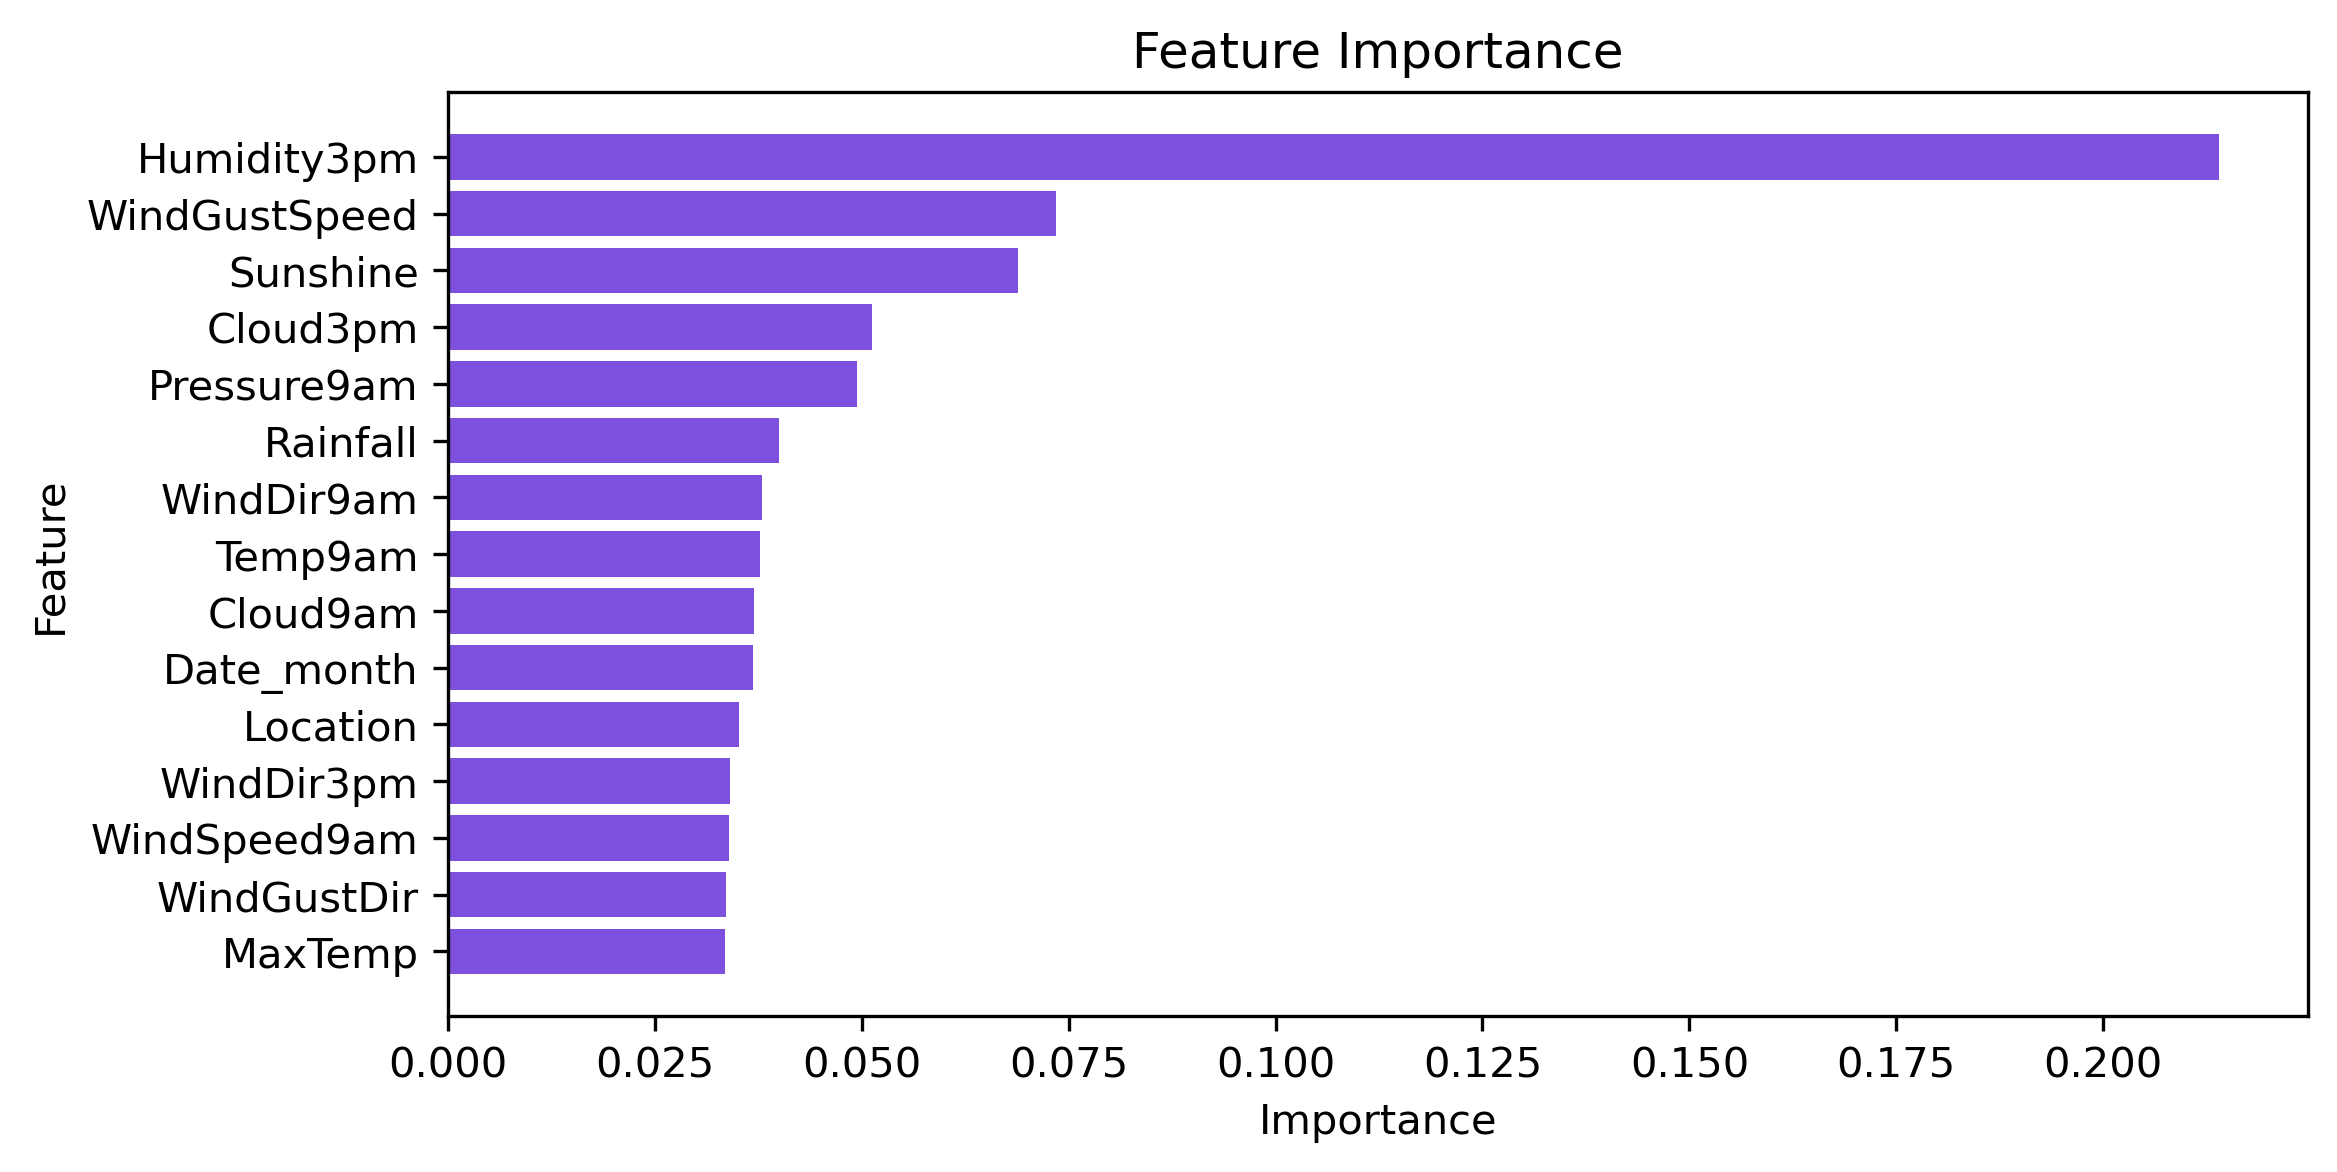
\includegraphics[width=350px]{XAI/XGBoost/feature_importance.png}%
\caption{Feature Importance for the best XGBoost model}%
\end{figure}

%


\begin{figure}[h!]%
\centering%
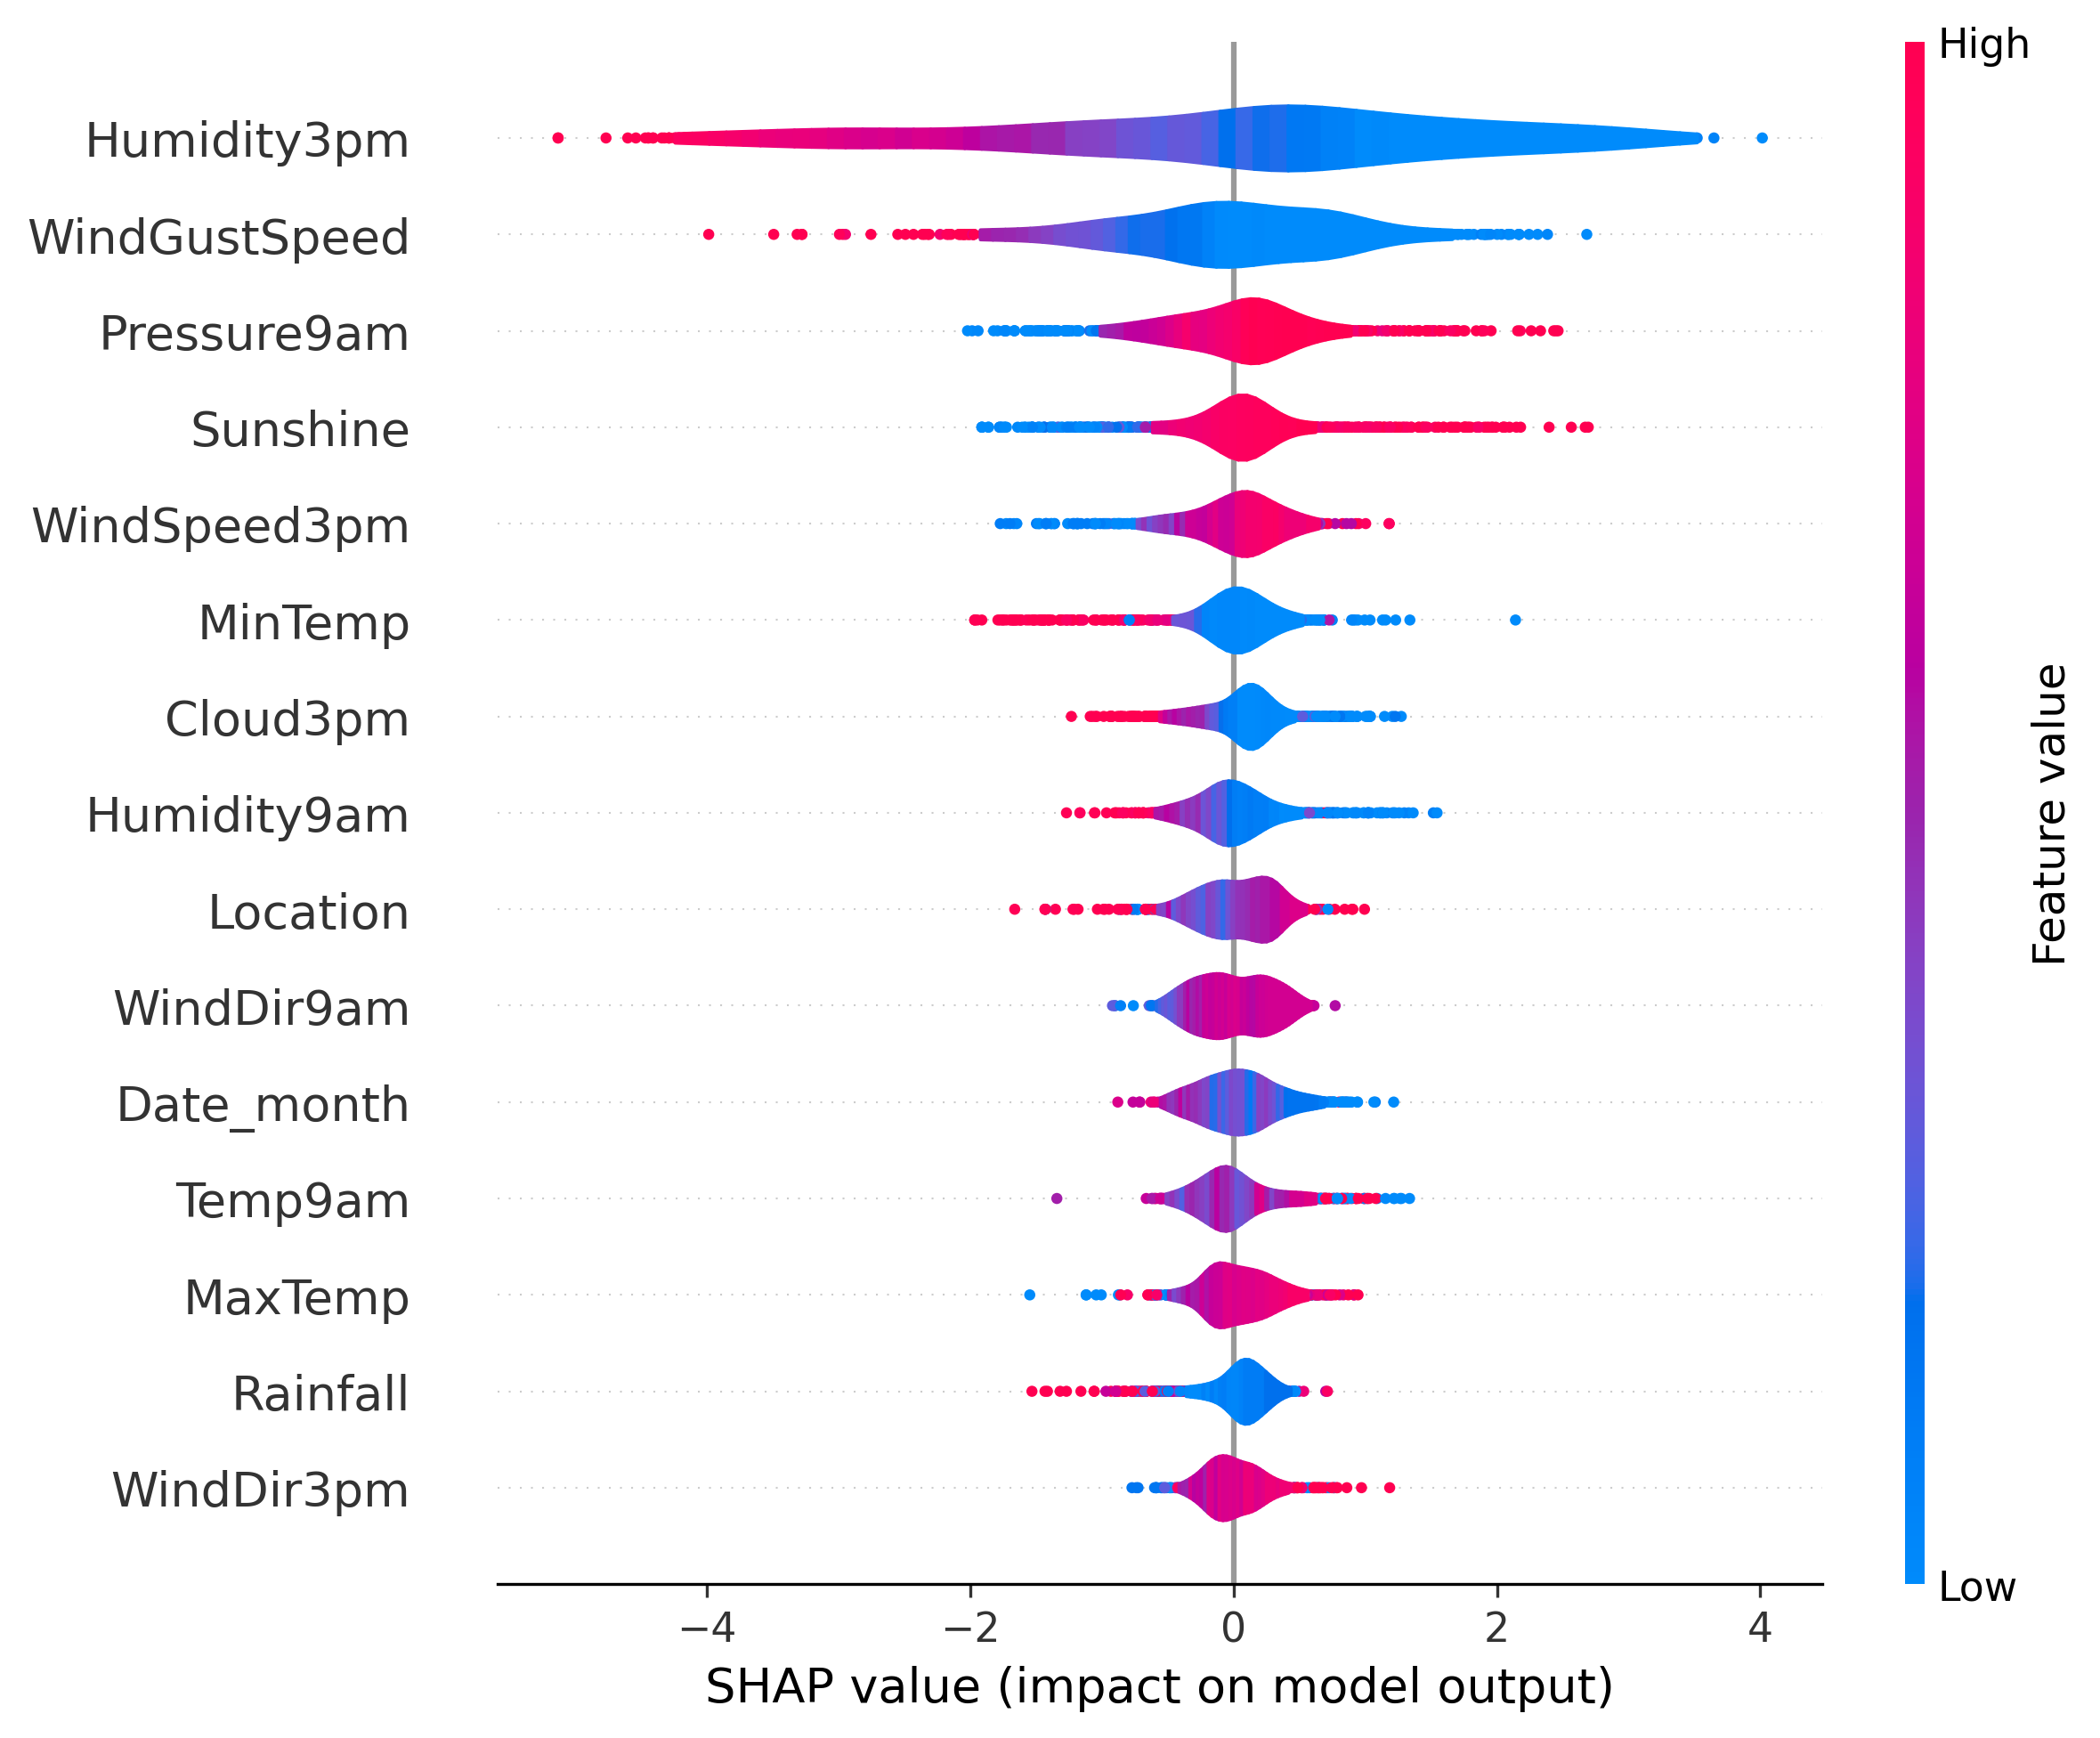
\includegraphics[width=400px]{XAI/XGBoost/violin_summary_plot_shap.png}%
\caption{Violin plot (SHAP) of impact on prediction for the best XGBoost model}%
\end{figure}

%
\end{document}